% article example for classicthesis.sty
\documentclass[10pt,a4paper]{article} % KOMA-Script article scrartcl
\usepackage{import}
\usepackage{xifthen}
\usepackage{pdfpages}
\usepackage{transparent}
\newcommand{\incfig}[1]{%
    \def\svgwidth{\columnwidth}
    \import{./figures/}{#1.pdf_tex}
}
\usepackage{lipsum}     %lorem ipsum text
\usepackage{titlesec}   %Section settings
\usepackage{titling}    %Title settings
\usepackage[margin=10em]{geometry}  %Adjusting margins
\usepackage{setspace}
\usepackage{listings}
\usepackage{amsmath}    %Display equations options
\usepackage{amssymb}    %More symbols
\usepackage{xcolor}     %Color settings
\usepackage{pagecolor}
\usepackage{mdframed}
\usepackage[spanish]{babel}
\usepackage[utf8]{inputenc}
\usepackage{longtable}
\usepackage{multicol}
\usepackage{graphicx}
\graphicspath{ {./Images/} }
\setlength{\columnsep}{1cm}

% ====| color de la pagina y del fondo |==== %



\begin{document}
    %========================{TITLE}====================%
    \title{{  12th laboratory  }}
    \author{{Rodrigo Castillo}}
    \date{\today}

    \maketitle


    %=======================NOTES GOES HERE===================%
    \section{2. Read the section "Introducción" from page 9 to 11 to describe
        in your own words each one of the 5 phases of an AFD (Análisis Forense
        Digital)}

        \begin{enumerate}
            \item {Identificación del incidente}
            \item {Recopilacion de evidencias}
            \item {preservación de la evidencia}
            \item {Análisis de la evidencia}
            \item {Documentación de los resultados}
        \end{enumerate}

        \textbf{identificación del incidente:}  consiste en identificar el problema, que puede ser : \begin{itemize}
                \item {un ataque de denegacion de sistema}
                \item {un malware}
                \item {una mala práctica de algún programador}
                \item {un backdoor en algun dispositivo}
        \end{itemize}

    \textbf{ Recopilación de evidencias} dependiendo del tipo de incidente, se
    recopilan evidencias que puedan conducir a juzgar al atacante, o a
    encontrar información que lleve hacia el.
    \\
    \textbf{preservación de la evidencia}  consiste en guardar la evidencia en
    algún lugar seguro.
    \\
    \textbf{Análisis de la eviencia} consiste en usar técnicas de análisis
    forense sobre la evidencia .
    \\
    \textbf{Documentación de los resultados} consiste en emitir un informe
    sobre los resultados del análisis de la envidencia.

    \section{Read the page 14, choose one of the described incidents and
    identify what would be the penalty for that incident according to the
    Colombian Law. For this answer review the Law 1273 here}

        \textbf{acceso abusivo a un sistema informático}: tiene pena de 48 a 96
        meses de prision y multa de 100 a 1000 salarios mínimos .
        \\
        \textbf{ataques de tipo DOS o DDOS}  tiene pena de 48 a 96
        meses de prision y multa de 100 a 1000 salarios mínimos .
        \\
        \textbf{ataques de tipo MITM :} pena de prisión de treinta y seis (36)
            a setenta y dos (72) meses.
        \\
        \textbf{ataques a bases de datos o a sistemas físicos}  pena de
            prisión de treinta y seis (48) a setenta y dos (96) meses y multa
            de 100 a 1000 salarios mínimos.
            \\
        \textbf{mi veredicto:}
        según entiendo, en el libro se describe un ataque de un gusano, por lo
        que yo lo definiría como acceso abusivo a un sistema informático , sin
        embargo, yo creo que la regulación de los ataques de tipo 0day es un
        poco ambigua, pues no necesariamente implican acceder de forma
        \textbf{abusiva}  a un sistema informático.

    \section{Read the section "Fases de un Análisis Forense Digital:
    Identificación del incidente" (Pages 15-20) and explain why may it be
    convenient to shutdown a computer unplugging it from the electrical outlet.}
        porque cuando se desconecta un computador se guarda el estado de la
        máquina o se congela, mientras que si se apaga manualmente se borra el
        contenido que está dentro de la memoria de acceso aleatorio

    \section{Read the section "Fases de un Análisis Forense Digital:
    Preservación de la evidencia" (Pages 20-21) and explain in your own word
    why it is important to get a hash value of the evidence?}

        es bueno calcularle el hash (en el texto dice que $MD5$ o $SHA1$ sin
        embargo no entiendo por que no usar algo como $SHA256$ ) , cada copia,
        llamarla con el nombre $COPIA-A$ y $COPIA-B$  o nombres sencillos de
        distinguir, con eso se puede guardar una copia infalseable de la
        información original obtenida.

    \section{Read the section "Fases de un Análisis Forense Digital: Análisis
    de la evidencia" (Pages 21-23) and explain in your own word the purpose of
    having a second pc with the exact configuration of the victim computer.}

        es importante para ver el cambio del computador victima de la manera
        exacta en la que cambió luego del ataque en un análisis dinámico tal
        cuál como aprendimos a hacerlo en el curso de análisis forense.


    \newpage
    \section{Recollection of evidence: Create a image of a Hard Disk or an USB}
        \begin{figure}[h!]
            \centering
            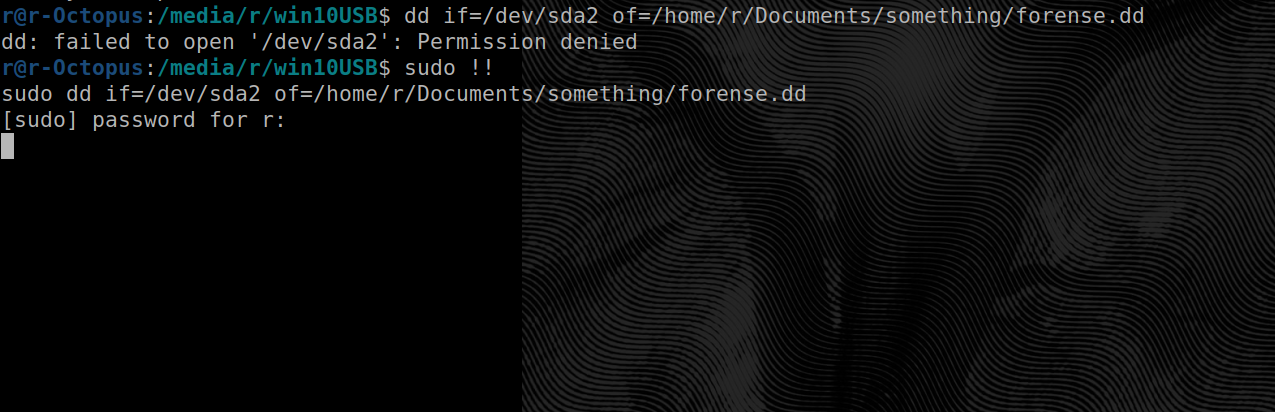
\includegraphics[width=0.8\linewidth]{sudo.png}
            \caption{copia bit a bit}
            \label{copia}
        \end{figure}

        en un proceso de una maquina que no fuera mia, no entiendo cómo
        funcionaría el proceso de recolección de evidencias sin la contraseña
        de superusuario.

        \begin{figure}[h!]
            \centering
            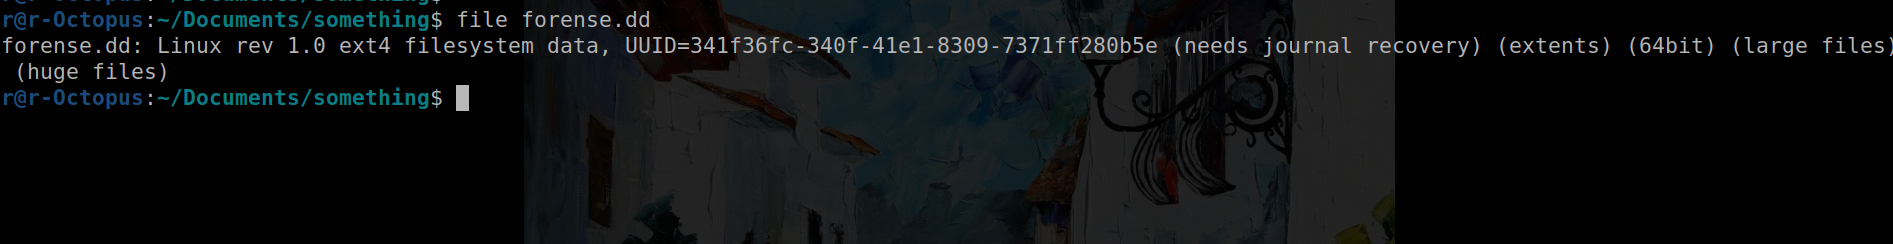
\includegraphics[width=0.8\linewidth]{tam.png}
            \caption{tamaño y tipo de archivo}
            \label{fig}
        \end{figure}

        \begin{figure}[h!]
            \centering
            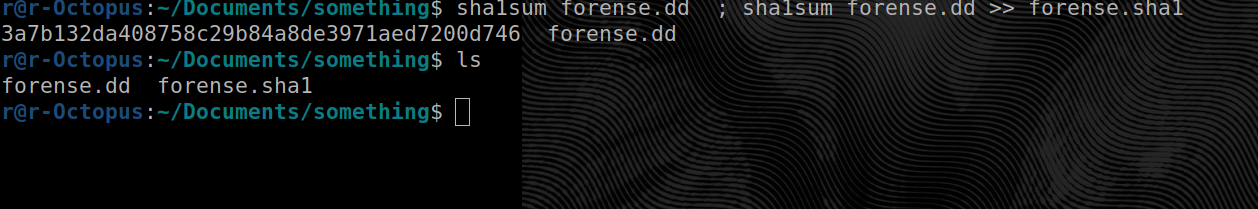
\includegraphics[width=0.8\linewidth]{sha1.png}
            \caption{sha1 y sha1 guardado}
            \label{fig}
        \end{figure}

        \color{red} Hola profe, llevo teniendo problemas con el instalador de
        Autopsy, por lo que voy a correrlo en otro sistema operativo en otro
        momento, y por ahora, entregaré el taller así , adjunto imagen del
        problema con el instalador de autopsy
        \color{black} .

        \begin{figure}[h!]
            \centering
            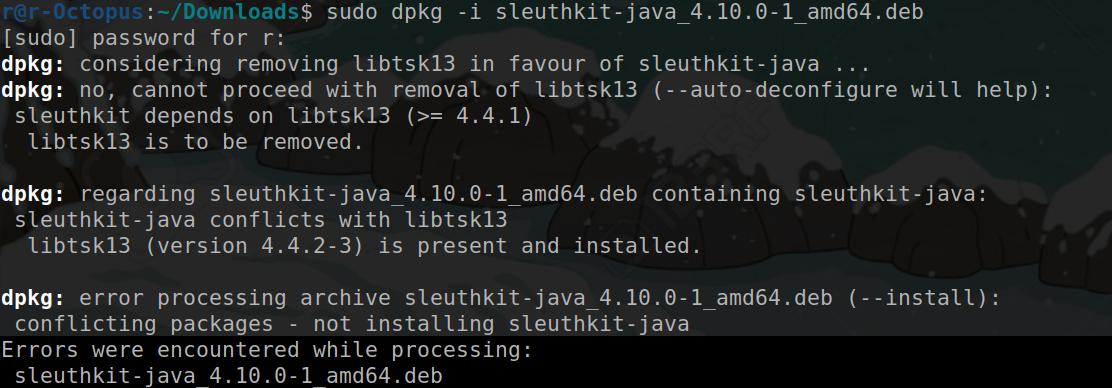
\includegraphics[width=0.8\linewidth]{autopsy.png}
            \caption{problema con el instalador de autopsy}
            \label{fig}
        \end{figure}

        sin embargo, no es la primera vez que uso autopsy, lo que debo hacer es
        buscar los archivos jpeg que están en el archivo $.dd$ que se encuentra
        en $http://dftt.sourceforge.net/test8/index.html$.
        \\
         Debido a que perdí
        la paciencia tratando de instalar autopsy , dejaré esta parte del
        taller para después.























    %=======================NOTES ENDS HERE===================%

    % bib stuff
    \nocite{*}
    \addtocontents{toc}{{}}
    \addcontentsline{toc}{section}{\refname}
    \bibliographystyle{plain}
    \bibliography{../Bibliography}
\end{document}
